\chapter{Introduction}\label{sec:intro}
\subsection{Motivation and Objectives}
Digital electronics\cite{DigialElectronics} is part of the most modern branch of electronics and is evolving rapidly nowadays mainly due to the advantages it offers and which will be analyzed in the present project. Therefore, it is important to bring this technology to the whole world, to make it friendly and provide society with the necessary tools for its correct understanding, without this implying of higher education achievement. \newline

Getting involved in a project not so developed and with lack of information, it may seem a bit overwhelming at first, especially when problems start to come out, but for any engineer it is quite a challenge to be able to start working on a determined field, offering society some useful tools for future implementations and improvements. \newline

Working on a platform native from Granada, Spain, such as the Ice-Zum Alhambra board, considering the lack of development in this field, is also an honor that should not be forgotten when it comes to naming the motivations and objectives. \newline

Digital electronics, FPGAs\cite{FPGAWhat}, microcontroller, hardware description \newline language\cite{HDL}, educational robotics\cite{6826237}, etc, are only some of the most important concepts on which this work is based and are also part of one of the most important research lines from engineers from all over the world. It is an objective to take this concept to the classrooms, specially to little kids, making use of the libraries of implementation hardware blocks that would help in the successive works and widening the educational robotic concept. \newline

The most important objectives from this work and which must be achieved are presented:
\begin{itemize}
	\item Ability to understand and implement all kinds of robotic behaviors through hardware implementation languages.
	\item Current robotic systems featuring.
	\item Open tools usage for educational robotics such as IceStudio.
	\item Ability to develop Printed Circuit Boards (PCB) with Altium Designer\cite{Altium}.
	\item Ability to design and construct mechanical structures by using SolidWorks\cite{SolidWorks} and 3D printers.
	\item Understating about the importance of the coexistence between Microcontroller and FPGA.
\end{itemize}
\subsection{Planification (Gantt Diagram)}

\begin{center}
	\begin{figure}[H]
		\center
		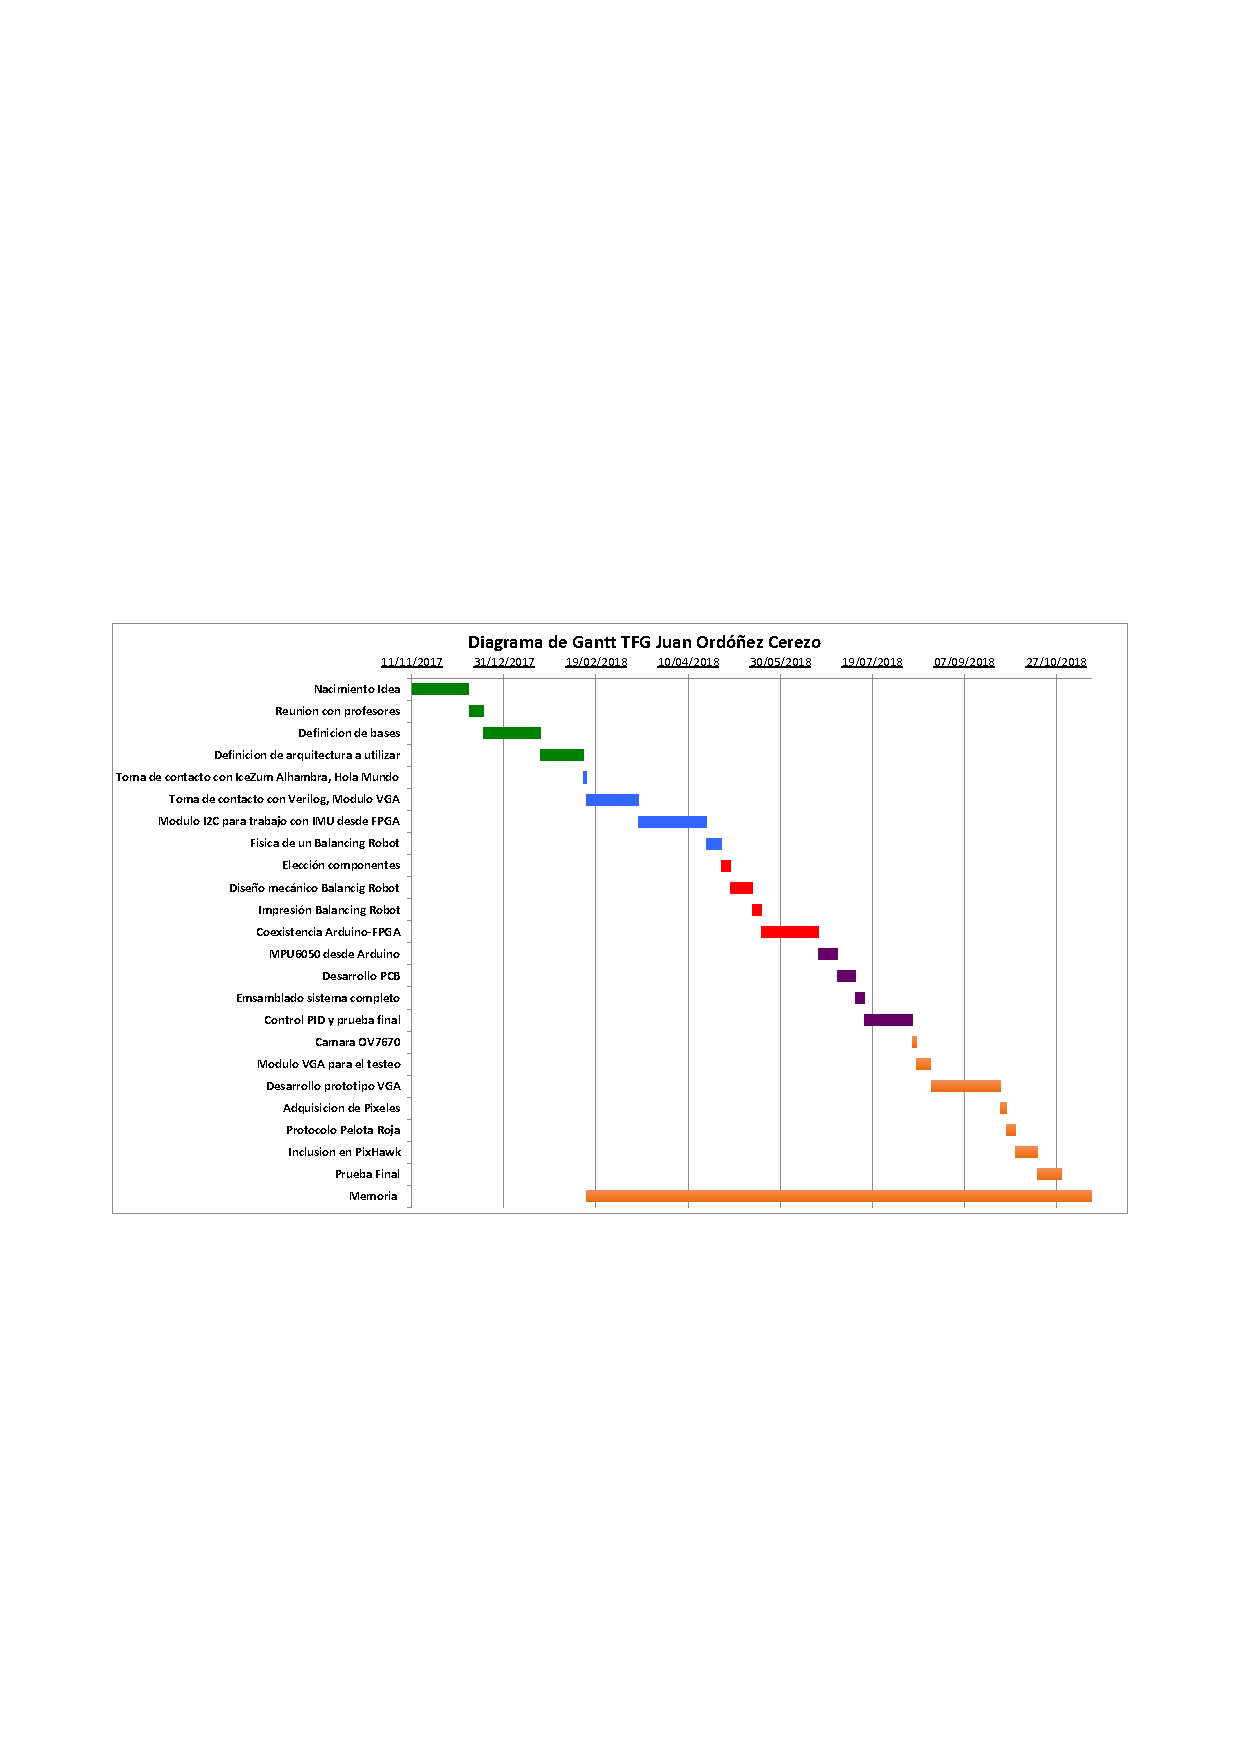
\includegraphics[trim = 15mm 85mm 2cm 100mm,clip, angle=-90, scale = 1]{imagenes/Introduction/Gantt.pdf}
		\label{fig:diagramaGantt}
		\caption{}
	\end{figure}
\end{center}

\subsection{Work Methodology}
In order to introduce the work methodology, GitHub tool will be introduced\cite{Git} (figure \ref{fig:github}).\newline 

\begin{figure}[H]
	\center
	
\includegraphics[trim = 0mm 0mm 0mm 0mm, clip,scale=0.4]{imagenes/Introduction/github}
	\caption{GitHub Logo.}
	\label{fig:github}
\end{figure}


GitHub is a collaborative software development platform for hosting projects using the Git version control system. GitHub hosts your project in a repository and provides very useful tools for teamwork.\newline
It also provides the possibility of a Wiki for the maintenance of the versions and information about them.\newline
In the present project GitHub has been used as a container, where everything has been partially uploaded, normally, when a stable version was obtained on any of the branches.\newline
This way, and to be wide open, anyone has been able to follow the progress of this, doubts, problems, or even use some of the modules or material uploaded.\newline
 
This project can be found at \cite{Repo_GitHub}. \newline  

An example of the trajectory of this project is represented in the screenshot of GitHub in Figure \ref{fig:capturaGit}.

\begin{figure}[H]
	\center
	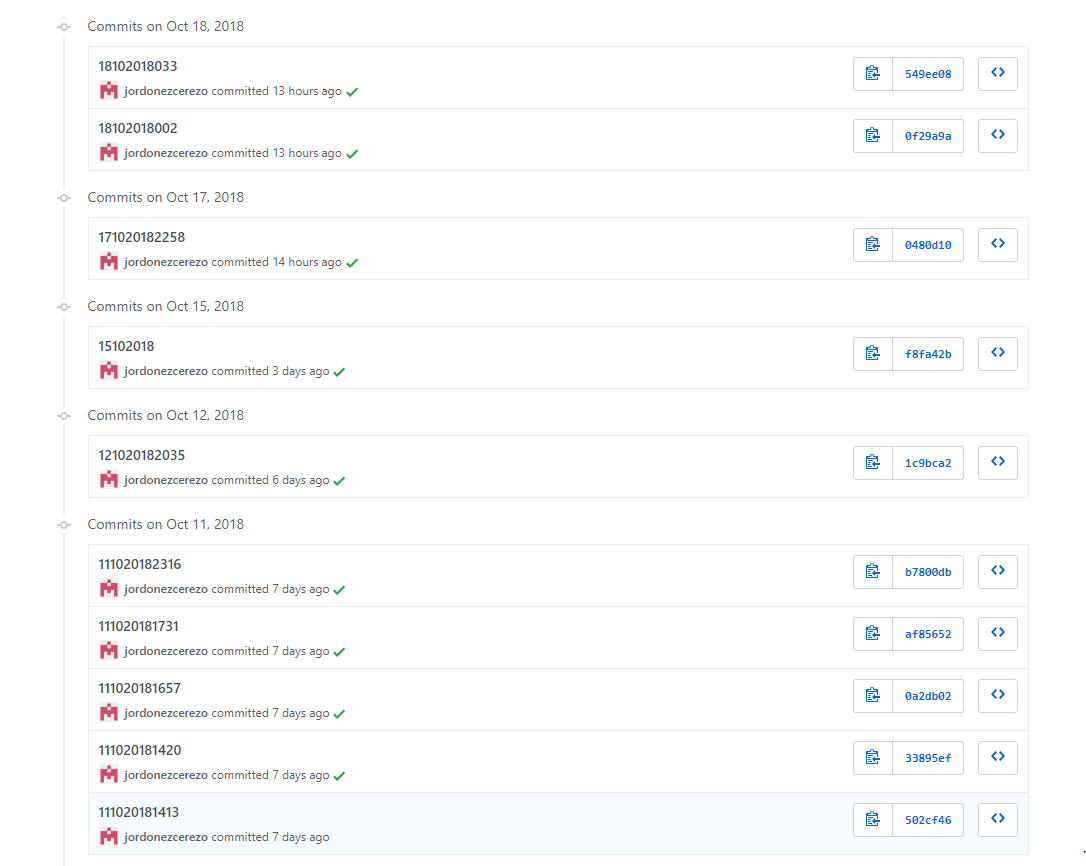
\includegraphics[trim = 0mm 0mm 0mm 0mm, clip,scale=0.5]{imagenes/Introduction/CapturaGit}
	\caption{Commits GitHub.}
	\label{fig:capturaGit}
\end{figure}

For the good fulfillment of the objectives settled out at first instance and taking into account the different location of the components of the work, it was necessary to propose weekly meetings (usually on Fridays) where the work done during the week was put together and new objectives were settled. \newline

For that, Appear.in\cite{Appear} tool, was used, which is a free software and offers videoconferences between several users at the same time.(figure \ref{fig:appear}). 

\begin{figure}[H]
	\center
	
\includegraphics[trim = 0mm 0mm 0mm 0mm, clip,scale=0.3]{imagenes/Introduction/appear}
	\caption{Appear.in.}
	\label{fig:appear}
\end{figure}

\subsection{Memory Structure}

Memory is divides in three chapters or differenced sections. \newline
In section \ref{sec:Estado_arte} will be briefly explained the whole theoretical part and basic knowledges for the understanding of this project. Also, the evolution through nowadays of some proposed systems will be commented.\newline

In section 3 \ref{sec: BalancingRobot} the Balancing Robot problem would be covered and a design part and an implementation part will be differentiated. The self-balance robot will be able to stay stable on two horizontal wheels.\newline

In section \ref{sec: Cuadricoptero} the vision problem on board a quad-copter will be covered as a first aproximation. \newline

At last but not least, in section \ref{sec: Conclusiones} conclusions from the whole work done will be exposed, as well as a possible future work to be done, errors to be corrected, etc.